\mySection{5.3 Interval Estimation}
%-------------- start slide -------------------------------%{{{ 5.34
\begin{frame}{\S\: 5.3 Interval Estimation}

 {\bf Rationale.~} Point estimate doesn't provide precision information. \\[1em]
  By using the variance of the estimator, one can construct \underline{an interval} such that with a \underline{\underline{high probability}} that interval will contain the unknown parameter.
 \\[1em]
 \begin{itemize}
  \item The \underline{interval} is called {\bf confidence interval}.\\[1em]
  \item The \underline{\underline{high probability}} is {\bf confidence level}.
 \end{itemize}
 \end{frame}

 \begin{frame}
\begin{enumerate}
 \item[E.g. 1.] A random sample of size $4$, ($Y_1 = 6.5$, $Y_2=9.2$, $Y_3=9.9$, $Y_4=12.4$),  from a normal population:
 \[
 f_Y(y;\mu) = \frac{1}{\sqrt{2\pi} \: 0.8} e^{-\frac{1}{2}\left(\frac{y-\mu}{0.8}\right)^2}.
 \]
 Both MLE and MME give $\mu_e = \bar{y} = \frac{1}{4}(6.5+9.2+9.9+12.4)=9.5$.
 The estimator $\widehat\mu=\overline{Y}$ follows normal distribution. \\[3em]
 Construct $95\%$-confidence interval for $\mu$ ...
\end{enumerate}
\end{frame}
%-------------- end slide -------------------------------%}}}
%-------------- start slide -------------------------------%{{{ 5.35
\begin{frame}
\begin{quotation}
  ``The parameter is an unknown constant and no probability statement concerning its value may be made." \\[1em]
--Jerzy Neyman, original developer of confidence intervals.
\end{quotation}
 \vfill
 \begin{center}
  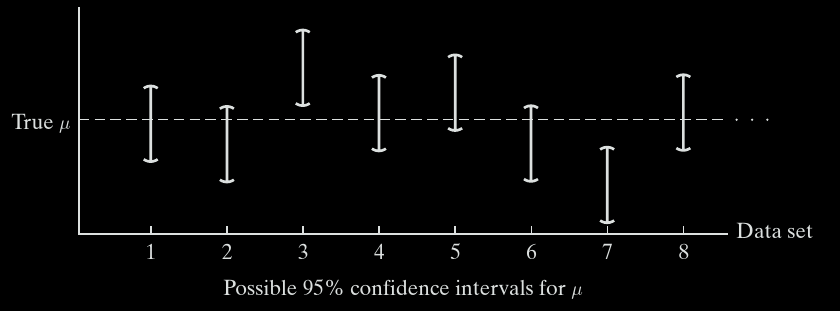
\includegraphics[scale=0.35]{Figure-5-3-2-neg.png}
\end{center}
\end{frame}
%-------------- end slide -------------------------------%}}}
%-------------- start slide -------------------------------%{{{ 5.36
\begin{frame}
  In general, for a normal population with $\sigma$ known, the {\bf $100(1-\alpha)\%$ confidence interval} for $\mu$ is
  \[
  \left(\bar{y} - z_{\alpha/2}\frac{\sigma}{\sqrt{n}}, \bar{y} + z_{\alpha/2}\frac{\sigma}{\sqrt{n}}\right)
  \]
\vfill
\pause
Comment: There are many variations
\begin{enumerate}
 \item One-sided interval such as
 \[
 \left(\bar{y} - z_{\alpha}\frac{\sigma}{\sqrt{n}}, \bar{y} \right)
 \quad\text{or}\quad
 \left(\bar{y}, \bar{y} + z_{\alpha}\frac{\sigma}{\sqrt{n}}\right)
 \]
 \item $\sigma$ is unknown and sample size is small: \hfill $z$-score $\rightarrow$ $t$-score
 \item $\sigma$ is unknown and sample size is large: \hfill $z$-score by CLT\\[1em]
 \item Non-Gaussian population but sample size is large: \hfill  $z$-score by CLT
\end{enumerate}
\end{frame}
%-------------- end slide -------------------------------%}}}
%-------------- start slide -------------------------------%{{{ 5.37
\begin{frame}

{\bf Theorem.~} Let $k$ be the number of successes in $n$ independent trials, where $n$ is large and
$p = \PP(success)$ is unknown. An approximate $100(1-\alpha)\%$ confidence interval for $p$ is
the set of numbers
 \[
 \left(\frac{k}{n}-z_{\alpha/2} \sqrt{\frac{(k/n)(1-k/n)}{n}},\:\frac{k}{n}+z_{\alpha/2} \sqrt{\frac{(k/n)(1-k/n)}{n}}\right).
 \]
\pause
\vfill
Proof: It follows the following facts:
\begin{itemize}
  \item $X\sim$binomial$(n,p)$ iff $X=Y_1+\cdots+Y_n$, while $Y_i$ are i.i.d. Bernoulli$(p)$:
  \begin{align*}
    \E[Y_i] = p\quad\text{and}\quad \Var(Y_i)=p(1-p).
  \end{align*}
  \item {\bf Central Limit Theorem}: Let $W_1, W_2,\cdots, W_n$ be an sequence of i.i.d. random variables, whose distribution has mean $\mu$ and variance  $\sigma^2$, then
    \begin{align*}
      \frac{\sum_{i=1}^n W_i - n\mu}{\sqrt{n\sigma^2 }} \quad \text{{\it approximately} follows}\quad N(0,1),\quad \text{when $n$ is large.}
    \end{align*}
\end{itemize}
\end{frame}
%-------------- end slide -------------------------------%}}}
%-------------- start slide -------------------------------%{{{ 1
\begin{frame}[fragile]
\begin{itemize}
  \item When the sample size $n$ is large, by the central limit theorem,
    \begin{align*}
      \frac{\sum_{i=1}^n Y_i - np}{\sqrt{np(1-p)}}
      \quad \stackrel{\text{ap.}}{\sim}\quad  N(0,1)
    \end{align*}
    \pause
    \[||\hspace{5em}\phantom{a}\]
    \vspace{-1em}
    \begin{align*}
      \hspace{5em}
      \frac{X - np}{\sqrt{np(1-p)}} =
      \frac{\frac{X}{n} - p}{\sqrt{\frac{p(1-p)}{n} }} \approx
      \frac{\frac{X}{n} - p}{\sqrt{\frac{p_e(1-p_e)}{n} }}
    \end{align*}
    \pause
  \item Since $p_e=\frac{k}{n}$, we see that
  \begin{align*}
    \mathbb{P}\left(-z_{\alpha/2} \le \frac{\frac{X}{n} - p}{\sqrt{\frac{\frac{k}{n}\left(1-\frac{k}{n}\right)}{n} }} \le z_{\alpha/2} \right) \approx 1-\alpha
  \end{align*}
  \item[] i.e., the $100(1-\alpha)\%$ confidence interval for $p$ is
 \[
 \left(\frac{k}{n}-z_{\alpha/2} \sqrt{\frac{(k/n)(1-k/n)}{n}},\:\frac{k}{n}+z_{\alpha/2} \sqrt{\frac{(k/n)(1-k/n)}{n}}\right).
 \]
 \myEnd
\end{itemize}
\end{frame}
%-------------- end slide -------------------------------%}}}
%-------------- start slide -------------------------------%{{{ 5.38
\begin{frame}

 \begin{enumerate}
  \item[E.g. 1.] Use {\it median test} to check the randomness of a random generator. \\[1em]
  \begin{quote}
   Suppose $y_1 , \cdots, y_n$ denote measurements presumed to have come from a
continuous pdf $f_Y(y)$. Let $k$ denote the number of $y_i$'s that are less than the median
of $f_Y (y)$. If the sample is random, we would expect the difference between $\frac{k}{n}$ and $\frac{1}{2}$
to be small. More specifically, a 95\% confidence interval based on $k$ should contain the value 0.5.
  \end{quote}
  \vfill
  \pause
  Let $f_Y(y)=e^{-y}$. The median is $m=0.69315$.
 \end{enumerate}

\end{frame}
%-------------- end slide -------------------------------%}}}
%-------------- start slide -------------------------------%{{{ 5.39
\begin{frame}[fragile]
 \begin{lstlisting}
#! /usr/bin/Rscript
main <- function() {
  args <- commandArgs(trailingOnly = TRUE)
  n <- 100 # Number of random samples.
  r <- as.numeric(args[1]) # Rate of the exponential
  # Check if the rate argument is given.
  if (is.na(r)) return("Please provide the rate and try again.")

  # Now start computing ...
  f <- function (y) pexp(y, rate = r)-0.5
  m <- uniroot(f, lower = 0, upper = 100, tol = 1e-9)$root
  print(paste("For rate ", r, "exponential distribution,",
              "the median is equal to ", round(m,3)))
  data <- rexp(n,r) # Generate n random samples
  data <- round(data,3) # Round to 3 digits after decimal
  data <- matrix(data, nrow = 10,ncol = 10) # Turn the data to a matrix
  prmatrix(data) # Show data on terminal
  k <- sum(data > m) # Count how many entries is bigger than m
  lowerbd = k/n  - 1.96 * sqrt((k/n)*(1-k/n)/n);
  upperbd = k/n  + 1.96 *sqrt((k/n)*(1-k/n)/n);
  print(paste("The 95% confidence interval is (",
              round(lowerbd,3), ",",
              round(upperbd,3), ")"))
}
main()
\end{lstlisting}
Try commandline ...
\end{frame}
%-------------- end slide -------------------------------%}}}
%-------------- start slide -------------------------------%{{{ 5.40
\begin{frame}
 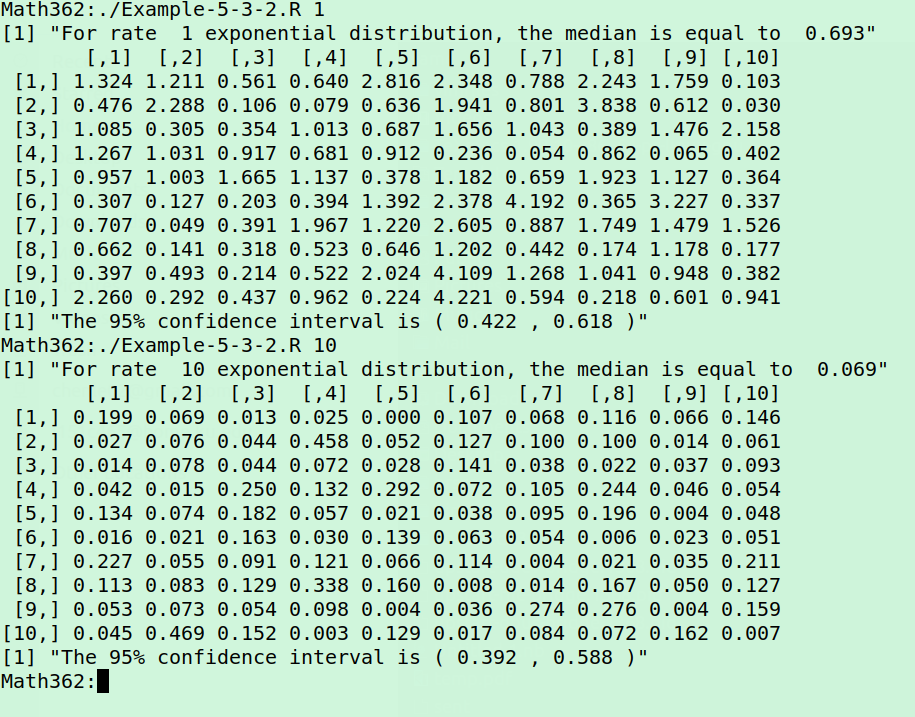
\includegraphics[scale=0.3]{Example-5-3-2-neg.png}
\end{frame}
%-------------- end slide -------------------------------%}}}
%-------------- start slide -------------------------------%{{{ 5.41
\begin{frame}
Instead of the C.I. $\left(\frac{k}{n}-z_{\alpha/2} \sqrt{\frac{(k/n)(1-k/n)}{n}},\:\frac{k}{n}+z_{\alpha/2} \sqrt{\frac{(k/n)(1-k/n)}{n}}\right)$.\\[1em]
One can simply specify the mean $\displaystyle \frac{k}{n}$ and
\[
\text{the {\bf margin of error}:}\qquad  d:=z_{\alpha/2} \sqrt{\frac{(k/n)(1-k/n)}{n}}.
\]
\vfill
\[
\max_{p\in(0,1)} p(1-p)  = p(1-p)\bigg|_{p=1/2} = 1/4 \quad \Longrightarrow \quad d\le \frac{z_{\alpha/2}}{2\sqrt{n}}=:d_m.
\]
\end{frame}
%-------------- end slide -------------------------------%}}}
%-------------- start slide -------------------------------%{{{ 5.42
\begin{frame}
 Comment:
 \begin{enumerate}
  \item When $p$ is close to $1/2$, $d\approx \frac{z_{\alpha/2}}{2\sqrt{n}}$, which is equivalent to $\sigma_p\approx \frac{1}{2\sqrt{n}}$.\\[1em]
 E.g., $n=1000$, $k/n=0.48$, and $\alpha=5\%$, then
 \[
 d=1.96\sqrt{\frac{0.48\times 0.52}{1000}} = 0.0309\underline{7} \quad \text{and}\quad
 d_m = \frac{1.96}{2\sqrt{1000}}= 0.0309\underline{9}
 \]
 \[
 \sigma_p = \sqrt{\frac{0.48\times 0.52}{1000}} =  0.015\underline{7}9873
 \quad \text{and}\quad
 \sigma_p \approx \frac{1}{2\sqrt{1000}}= 0.015\underline{8}1139.
 \]
 \vfill
 \item When $p$ is away from $1/2$, the discrepancy between $d$ and $d_m$ becomes big....
\end{enumerate}
\end{frame}
%-------------- end slide -------------------------------%}}}
%-------------- start slide -------------------------------%{{{ 5.43
\begin{frame}
 \begin{enumerate}
  \item[E.g. ]  Running for presidency. Max and Sirius obtained 480 and 520 votes, respectively. What is probability that Max will win?
  \vfill
  What if the sample size is $n=5000$, and Max obtained 2400 votes.
 \end{enumerate}
\end{frame}
%-------------- end slide -------------------------------%}}}
%-------------- start slide -------------------------------%{{{ 5.44
\begin{frame}{Choosing sample sizes}

 \begin{align}
   d \le  z_{\alpha/2} \sqrt{p(1-p)/n} &\quad\Longleftrightarrow\quad n \ge \frac{z_{\alpha/2}^2p(1-p)}{d^2} \tag{When $p$ is known} \\[1em]
 d \le \frac{z_{\alpha/2}}{2\sqrt{n}} &\quad\Longleftrightarrow\quad n \ge \frac{z_{\alpha/2}^2}{4d^2} \tag{When $p$ is unknown}
 \end{align}
\vfill
\begin{enumerate}
 \item[E.g. ]  Anti-smoking campaign. Need to find an $95\%$ C.I.  with a margin of error equal to $1\%$. Determine the sample size? \\[1em]
 Answer: $n\ge \frac{1.96^2}{4\times 0.01^2} = 9640$.
 \vfill
 \item[E.g.'] In order to reduce the sample size, a small sample is used to determine $p$. One finds that $p\approx 0.22$. Determine the sample size again. \\[1em]
 Answer: $n\ge \frac{1.96^2 \times 0.22\times 0.78}{\times 0.01^2} = 6592.2$.
\end{enumerate}
\end{frame}
%-------------- end slide -------------------------------%}}}
